\documentclass[hyperref={pdfpagelabels=false},aspectratio=169]{beamer}
\usepackage{lmodern}
\usetheme{CambridgeUS}

\usepackage[utf8]{inputenc}
\usepackage[english]{babel}
\usepackage{graphicx} 
\usepackage{xcolor}
\usepackage{spverbatim}
\usepackage{pgf-pie}
%\usepackage{bibgerm}

\usepackage{mwe,tikz}\usepackage[percent]{overpic}

\usepackage{appendixnumberbeamer}

\usepackage{pdfpages}
\usepackage{adjustbox}
\usepackage{stmaryrd}
\usepackage{graphicx,caption}
\usepackage{multirow}
\usepackage{graphicx}
\usepackage{ulem}
\usepackage{filecontents}

\setbeamertemplate{navigation symbols}{}%remove navigation symbols


% custom variables
\newcommand{\allClaimsInCorpus}{\mathcal{C}}
\newcommand{\claimCluster}{\gamma}
\newcommand{\allClaimClustersInCorpus}{\Gamma}

\newcommand{\allPremisesInCorpus}{\mathcal{P}}
\newcommand{\premiseCluster}{\pi}
\newcommand{\allPremiseClustersInCorpus}{\Pi}
\newcommand{\allDimensionsThatExists}{\mathcal{D}}
\newcommand{\allDimensionsThatAreChosen}{\Delta}

\newcommand{\alignedStances}{q\!\uparrow \uparrow\!c}
\newcommand{\notAlignedStances}{q\!\uparrow \downarrow\!c}

\newcommand{\pf}{\textsl{pf}}
%\newcommand{\cf}{\textsl{cf}}
\newcommand{\icf}{\textsl{icf}}
\newcommand{\pfIcf}{\textsl{pfIcf}}
\newcommand{\dcf}{\textsl{dcf}}
\newcommand{\avg}{\textsl{avg}}
\newcommand{\tfIdf}{\textsc{tf-idf}}
\newcommand{\co}{\textsc{co}}
\newcommand{\re}{\textsc{re}}
\newcommand{\ef}{\textsc{ef}}

\newcommand{\datasetEnergy}{dataset$_{\textsl{energy}}$}
\newcommand{\datasetSpread}{dataset$_{\textsl{spread}}$}

\newcommand{\mycomment}[1]{}


% http://www.computerhope.com/htmcolor.htm
\definecolor{blueGray}{HTML}{98AFC7}
\definecolor{seaBlue}{HTML}{C2DFFF}
\definecolor{aliceBlue}{HTML}{F0F8FF}
\definecolor{lapisBlue}{HTML}{15317E}
\definecolor{transperencygray}{rgb}{0.9, 0.9, 0.9}


\definecolor{mybackground}{HTML}{FFA500}
\definecolor{myforeground}{HTML}{000000}

\setbeamercolor{normal text}{fg=black,bg=white}
\setbeamercolor{alerted text}{fg=red}
\setbeamercolor{example text}{fg=olive}

\setbeamercolor{background canvas}{fg=myforeground, bg=white}
\setbeamercolor{background}{fg=myforeground, bg=mybackground}

\setbeamercolor{palette primary}{fg=black, bg=aliceBlue}
\setbeamercolor{palette secondary}{fg=black, bg=seaBlue}
\setbeamercolor{palette tertiary}{fg=black, bg=blueGray}

\setbeamercolor{frametitle}{fg=lapisBlue}
\setbeamercolor{title}{fg=lapisBlue}


\theoremstyle{definition}
\newtheorem{mydef}[theorem]{Definition}


\usepackage{lipsum}
\usepackage{picture}
\usepackage{todonotes}
\usepackage{listings}
\usepackage{pgf-pie}
\usepackage{spverbatim}
\usepackage{eso-pic}
\usepackage{amsfonts} 
\usepackage{algorithm}
\usepackage{algpseudocode}

\newcommand\blfootnote[1]{%
  \begingroup
  \renewcommand\thefootnote{}\footnote{#1}%
  \addtocounter{footnote}{-1}%
  \endgroup
}

\setbeamerfont{title}{size=\large}

% Wasserzeichen
\usepackage{eso-pic}
\newcommand\BackgroundPic{%
\put(0,0){%
\parbox[b][\paperheight]{\paperwidth}{%
\vfill
\centering
\begin{figure}  
  \begin{overpic}[scale=1.5]{img/wasserzeichen.jpg}
     \put(-30,0){
\includegraphics[scale=0.05]{img/uniLogo2.png}}
  \end{overpic}
\end{figure}
\vfill
}}}

\usebackgroundtemplate%

\title[Bachelor Thesis]{The Track Layout Problem from a
SAT-Solving Perspectives}
\author{Simon Szulik}
\institute[ ]{
Advisors:\\
Jun.-Prof.~Dr.~Philipp~Kindermann\\
Prof.~Dr.~Stefan~Näher\\
}
\date{\today}


\begin{document}

\AddToShipoutPicture*{\BackgroundPic}


% F1
\begin{frame}
\titlepage
\end{frame} 

\begin{frame}{Track-Layout}
    \begin{columns}
        \begin{column}{0.5\textwidth}
            „A track layout of a graph is a partition of its vertices into sequences, called tracks, such that the vertices in each sequence form an independent set and the edges between each two pairs of tracks form a non-crossing set” \sim Dujmović \, et \, al.
        \end{column}
        \begin{column}{0.5\textwidth}
            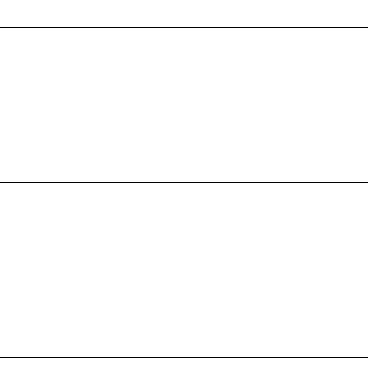
\includegraphics[scale=0.7]{img/octahedron_tlp_nur_tracks.png}
        \end{column}
    \end{columns}
\end{frame}

\begin{frame}{Track-Layout}
    \begin{columns}
        \begin{column}{0.5\textwidth}
            „A track layout of a graph is a partition of its vertices into sequences, called tracks, such that the vertices in each sequence form an independent set and the edges between each two pairs of tracks form a non-crossing set” \sim Dujmović \, et \, al.
        \end{column}
        \begin{column}{0.5\textwidth}
            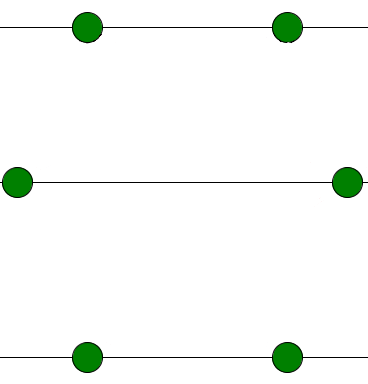
\includegraphics[scale=0.7]{img/octahedron_tlp_3_tracks.png}
        \end{column}
    \end{columns}
\end{frame}

\begin{frame}{Track-Layout}
    \begin{columns}
        \begin{column}{0.5\textwidth}
            „A track layout of a graph is a partition of its vertices into sequences, called tracks, such that the vertices in each sequence form an independent set and the edges between each two pairs of tracks form a non-crossing set” \sim Dujmović \, et \, al.
        \end{column}
        \begin{column}{0.5\textwidth}
            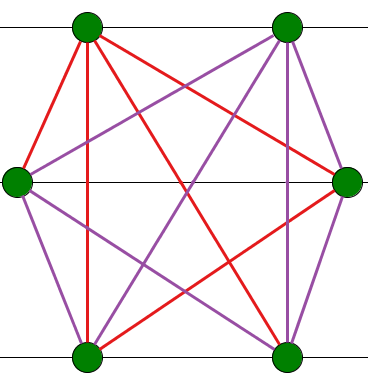
\includegraphics[scale=0.7]{img/octahedron_tlp_ganz.png}
        \end{column}
    \end{columns}
\end{frame}

\begin{frame}{Rules}
\begin{columns}
    \begin{column}{0.5\textwidth}
        \begin{itemize}
            \item \textbf{Uniqueness}: Each node exists only once and is positioned on exactly one track
        \end{itemize}
    \end{column}
    \begin{column}{0.5\textwidth}
    \end{column}
\end{columns}
\end{frame}

\begin{frame}{Rules}
\begin{columns}
    \begin{column}{0.5\textwidth}
        \begin{itemize}
            \item \textbf{Uniqueness}: Each node exists only once
            \item \textbf{Adjacent Nodes}: Adjacent nodes must not be on the same track
        \end{itemize}
    \end{column}
    \begin{column}{0.5\textwidth}
    \end{column}
\end{columns}
\end{frame}

\begin{frame}{Rules}
\begin{columns}
    \begin{column}{0.5\textwidth}
        \begin{itemize}
            \item \textbf{Uniqueness}: Each node exists only once
            \item \textbf{Adjacent Nodes}: Adjacent nodes must not be on the same track
            \item \textbf{Problem Definition}: Let $L$ be a correct Layout for $G$ and $F(G, t)$ evaluate to true if an $L$ for $G$ with $t$ tracks exists
        \end{itemize}
    \end{column}
    \begin{column}{0.5\textwidth}
    \end{column}
\end{columns}
\end{frame}

\begin{frame}{Rules}
\begin{columns}
    \begin{column}{0.5\textwidth}
        \begin{itemize}
            \item \textbf{Uniqueness}: Each node exists only once
            \item \textbf{Adjacent Nodes}: Adjacent nodes must not be on the same track
            \item \textbf{Problem Definition}: Let $L$ be a correct Layout for $G$ and $F(G, t)$ evaluate to true if an $L$ for $G$ with $t$ tracks exists
        \end{itemize}
    \end{column}
    \begin{column}{0.5\textwidth}
        \vspace{2cm}
        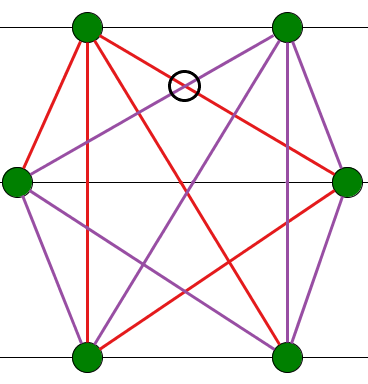
\includegraphics[scale=0.6]{img/Regeln_1.png}
    \end{column}
\end{columns}
\end{frame}

\begin{frame}{Rules}
\begin{columns}
    \begin{column}{0.5\textwidth}
        \begin{itemize}
            \item \textbf{Uniqueness}: Each node exists only once
            \item \textbf{Adjacent Nodes}: Adjacent nodes must not be on the same track
            \item \textbf{Problem Definition}: Let $L$ be a correct Layout for $G$ and $F(G, t)$ evaluate to true if an $L$ for $G$ with $t$ tracks exists
        \end{itemize}
    \end{column}
    \begin{column}{0.5\textwidth}
        \vspace{2cm}
        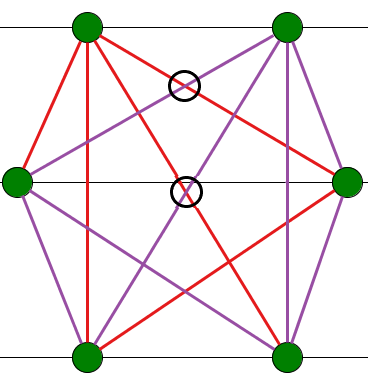
\includegraphics[scale=0.6]{img/Regeln_2.png}
    \end{column}
\end{columns}
\end{frame}

\begin{frame}{Rules}
\begin{columns}
    \begin{column}{0.5\textwidth}
        \begin{itemize}
            \item \textbf{Uniqueness}: Each node exists only once
            \item \textbf{Adjacent Nodes}: Adjacent nodes must not be on the same track
            \item \textbf{Problem Definition}: Let $L$ be a correct Layout for $G$ and $F(G, t)$ evaluate to true if an $L$ for $G$ with $t$ tracks exists
        \end{itemize}
    \end{column}
    \begin{column}{0.5\textwidth}
        \vspace{2cm}
        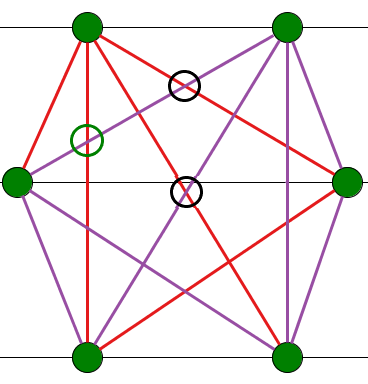
\includegraphics[scale=0.6]{img/Regeln_3.png}
    \end{column}
\end{columns}
\end{frame}

\begin{frame}{TLP Definitions}
    \begin{columns}
        \begin{column}{1\textwidth}
            \begin{itemize}
            \item \textbf{Graph Definition}: Let $G = (V,E)$ be the graph, $V =\{v_1,v_2,...,v_n\}$ be the vertices, $E = \{e_1,e_2,...,e_n\}$ be the edges.
            \end{itemize}
        \end{column}
    \end{columns}
\end{frame}

\begin{frame}{TLP Definitions}
    \begin{columns}
        \begin{column}{1\textwidth}
            \begin{itemize}
            \item \textbf{Graph Definition}: Let $G = (V,E)$ be the graph, $V =\{v_1,v_2,...,v_n\}$ be the vertices, $E = \{e_1,e_2,...,e_n\}$ be the edges.
            \item \textbf{Problem Definition}: Let $L$ be a correct Layout for $G$ and $F(G, t)$ evaluate to true if an $L$ for $G$ with $t$ tracks exists
            \end{itemize}
        \end{column}
    \end{columns}
\end{frame}

\begin{frame}{SAT Formulation \& Base Variables}
    \begin{columns}
        \begin{column}{1\textwidth}
            \begin{itemize}
            \item \textbf{Assigning nodes}: $\sigma(v_i,t_k)$ for each pair of nodes $v_i \in V$ and track $t$
            \end{itemize}
        \end{column}
    \end{columns}
\end{frame}

\begin{frame}{SAT Formulation \& Base Variables}
    \begin{columns}
        \begin{column}{1\textwidth}
            \begin{itemize}
            \item \textbf{Assigning nodes}: $\sigma(v_i,t_k)$ for each pair of nodes $v_i \in V$ and track $t$
            \newline
            \newline
            \cdot  \,  $(\sigma(v_i,t_1) \lor \sigma(v_i,t_2) \lor \dots \lor \sigma(v_i,t_n)) \, \forall v_i \in V \text{ and every track }t $ 
            \end{itemize}
        \end{column}
    \end{columns}
\end{frame}

\begin{frame}{SAT Formulation \& Base Variables}
    \begin{columns}
        \begin{column}{1\textwidth}
            \begin{itemize}
            \item \textbf{Assigning nodes}: $\sigma(v_i,t_k)$ for each pair of nodes $v_i \in V$ and track $t$
            \newline
            \newline
            \cdot  \, $ (\sigma(v_i,t_1) \lor \sigma(v_i,t_2) \lor \dots \lor \sigma(v_i,t_n)) \, \forall v_i \in V \text{ and every track }t $
            \newline
            \newline
            \cdot  \, $ (\overline{\sigma(v_i, t_x) \land \sigma(v_i, t_y)}) \, \forall v_i \in V \text{ and every combination of two tracks } x, y \text{ with } x \neq y$
            \end{itemize}
        \end{column}
    \end{columns}
\end{frame}

\begin{frame}{SAT Formulation \& Base Variables}
    \begin{columns}
        \begin{column}{1\textwidth}
            \begin{itemize}
            \item \textbf{Assigning nodes}: $\sigma(v_i,t_k)$ for each pair of nodes $v_i \in V$ and track $t$
            \newline
            \newline
            \cdot  \, $ (\sigma(v_i,t_1) \lor \sigma(v_i,t_2) \lor \dots \lor \sigma(v_i,t_n)) \, \forall v_i \in V \text{ and every track }t $
            \newline
            \newline
            \cdot  \, $ (\overline{\sigma(v_i, t_x) \land \sigma(v_i, t_y)}) \, \forall v_i \in V \text{ and every combination of two tracks } x, y \text{ with } x \neq y$
            \newline
            \item \textbf{Adjacency Rule}: $ \forall e_{i,j} \in E : (\overline{\sigma(v_i,t_x) \land \sigma(v_j,t_x)}) \text{ for every track } t $
            \end{itemize}
        \end{column}
    \end{columns}
\end{frame}

\begin{frame}{SAT Formulation \& Crossing Edges (Intuitive Approach)}
    \begin{columns}
        \begin{column}{1\textwidth}
        \end{column}
    \end{columns}
\end{frame}

\begin{frame}{SAT Formulation \& Crossing Edges (Intuitive Approach)}
    \begin{columns}
        \begin{column}{1\textwidth}
            \begin{itemize}
                \item \textbf{Position Numbers}: $\phi(v_i,p)$ for each $v_i \in V$ and every position $p$
            \end{itemize}
        \end{column}
    \end{columns}
\end{frame}

\begin{frame}{SAT Formulation \& Crossing Edges}
    \begin{columns}
        \begin{column}{1\textwidth}
            \begin{itemize}
                \item \textbf{Position Numbers}: $\phi(v_i,p)$ for each $v_i \in V$ and every position $p$
                \item \textbf{Forbid crossings}: $ \forall e_{i,j}, e_{u,w} \in E, \ \forall m,n,a,b \text{ in range of } \vert V \vert \text{ with } m<n, \, a<b,:$
                \newline
                \newline
                $(\overline{\sigma(v_i,t_x) \land \sigma(v_u,t_x) \land \sigma(v_j,t_y) \land \sigma(v_w,t_y) \land \phi(v_i,p_m) \land \phi(v_u,p_n) \land \phi(v_w,p_a) \land \phi(v_j,p_b)}$
                \newline
                \newline
                $\text{ for all disjoint pair of tracks } t_x \text{ and } t_y $
            \end{itemize}
        \end{column}
    \end{columns}
\end{frame}

\begin{frame}{SAT Formulation \& Crossing Edges (Relational Approach)}
    \begin{columns}
        \begin{column}{1\textwidth}
            \begin{itemize}
                \item \textbf{Relational Position}:  $\omega(v_i,v_j)$ for each $v_i,v_j \in V$
            \end{itemize}
        \end{column}
    \end{columns}
\end{frame} 

\begin{frame}{SAT Formulation \& Crossing Edges (Relational Approach)}
    \begin{columns}
        \begin{column}{1\textwidth}
            \begin{itemize}
                \item \textbf{Relational Position}:  $\omega(v_i,v_j)$ for each $v_i,v_j \in V$
                \newline
                \newline
                \cdot $ \omega(v_i,v_j) \leftrightarrow \lnot \omega(v_j,v_i) $
            \end{itemize}
        \end{column}
    \end{columns}
\end{frame}

\begin{frame}{SAT Formulation \& Crossing Edges (Relational Approach)}
    \begin{columns}
        \begin{column}{1\textwidth}
            \begin{itemize}
                \item \textbf{Relational Position}:  $\omega(v_i,v_j)$ for each $v_i,v_j \in V$
                \newline
                \newline
                \cdot $ \omega(v_i,v_j) \leftrightarrow \lnot \omega(v_j,v_i) $
                \newline
                \newline
                \cdot $ \omega(v_i,v_j) \land \omega(v_j,v_k) \rightarrow \omega(v_i,v_k) \, \forall \text{ pairwise distinct } v_i,v_j,v_k \in V$
            \end{itemize}
        \end{column}
    \end{columns}
\end{frame}

\begin{frame}{SAT Formulation \& Crossing Edges (Relational Approach)}
    \begin{columns}
        \begin{column}{1\textwidth}
            \begin{itemize}
                \item \textbf{Relational Position}:  $\omega(v_i,v_j)$ for each $v_i,v_j \in V$
                \newline
                \newline
                \cdot $ \omega(v_i,v_j) \leftrightarrow \lnot \omega(v_j,v_i) $
                \newline
                \newline
                \cdot $ \omega(v_i,v_j) \land \omega(v_j,v_k) \rightarrow \omega(v_i,v_k) \, \forall \text{ pairwise distinct } v_i,v_j,v_k \in V$
                \newline
                \newline
                \cdot $ \omega(v_i,v_j) \rightarrow \sigma(v_i,t_k) \land \sigma(v_j,t_k) \, \forall \text{ pairwise distinct } v_i,v_j \in V \text{and every track }t$
            \end{itemize}
        \end{column}
    \end{columns}
\end{frame}

\begin{frame}{SAT Formulation \& Crossing Edges (Relational Approach)}
    \begin{columns}
        \begin{column}{1\textwidth}
            \begin{itemize}
                \item \textbf{Relational Position}:  $\omega(v_i,v_j)$ for each $v_i,v_j \in V$
                \newline
                \newline
                \cdot $ \omega(v_i,v_j) \leftrightarrow \lnot \omega(v_j,v_i) $
                \newline
                \newline
                \cdot $ \omega(v_i,v_j) \land \omega(v_j,v_k) \rightarrow \omega(v_i,v_k) \, \forall \text{ pairwise distinct } v_i,v_j,v_k \in V$
                \newline
                \newline
                \cdot $ \omega(v_i,v_j) \rightarrow \sigma(v_i,t_k) \land \sigma(v_j,t_k) \, \forall \text{ pairwise distinct } v_i,v_j \in V \text{and every track }t$
                \newline
                \item \textbf{Forbid crossings}: $ \forall e_{i,j}, e_{u,w} \in E, \text{ and for all dosjoint pair of tracks $t_x$ and $t_y$ }:$
                \newline
                \newline
                $ \overline{(\sigma(v_i,t_x) \land \sigma(v_u,t_x) \land (\sigma(v_j,t_y) \land (\sigma(v_w,t_y) \land \omega(v_i,v_u) \land \omega(v_w,v_j)}$
            \end{itemize}
        \end{column}
    \end{columns}
\end{frame}

\begin{frame}{SAT Formulation \& Crossing Edges ("Improved" Relational Approach)}
    \begin{columns}
        \begin{column}{1\textwidth}
            \begin{itemize}
                \item \textbf{Extra Variable}: $\psi(v_i,v_j)$ for each $v_i,v_j \in V$
                \newline
                \newline
                \cdot $ \sigma(v_i,t_k) \land \sigma(v_j,t_k)\rightarrow \psi(v_i,v_j) \, \forall v_i,v_j \in V \text{and every track }t$
                \newline
                \item \textbf{Forbid crossings}: $ \forall e_{i,j}, e_{u,w} \in E : \overline{(\psi(v_i,v_u) \land \psi(v_j,v_w) \land   \omega(v_i,v_u) \land \omega(v_w,v_j)}$
            \end{itemize}
        \end{column}
    \end{columns}
\end{frame}

\begin{frame}{Hypotheses}
    \begin{columns}
        \begin{column}{1\textwidth}
            \begin{itemize}
                \item \textbf{H1}: Method 3 significantly reduces the clause number
                \item \textbf{H2}: The third approach will take less time to evaluate, depending on the number of clauses
            \end{itemize}
        \end{column}
    \end{columns}
\end{frame}

\begin{frame}{Environment \& Testdata}
    \begin{columns}
        \begin{column}{1\textwidth}
            \begin{itemize}
                \item \textbf{Implementation}: Python \& PySAT
                \item \textbf{SAT-Solver}: Lingeling
                \item \textbf{Data Benchmark}: Graph Layout Benchmark Datasets (Die Bartolomeo et al.) 
                \item \textbf{Dataset}: Rome-Lib (11534 graphs, 10 to 100 nodes, 9 to 158 edges) (Di Batista et al.)
            \end{itemize}
            \, \, \, \, \rightarrow \text{100 graphs with } 10 \times n \text{ nodes each}
        \end{column}
    \end{columns}
\end{frame}

\end{document}



                